\documentclass[12pt]{article}

\usepackage{geometry}
\geometry{a4paper, left=1in, right=1in, top=1in, bottom=1in}
\usepackage{amsmath}
\usepackage{amsmath,amsfonts,amssymb}
\usepackage{graphicx}
\usepackage{enumitem}
\usepackage{titlesec}
\usepackage{fancyhdr}
\usepackage{hyperref}
\usepackage{floatrow}
\usepackage{listings}
\usepackage{geometry}
\usepackage{fancyhdr}
\usepackage{empheq}
\usepackage[svgnames]{xcolor}
\usepackage{xpatch}

% Define MATLAB style for listings
\lstdefinestyle{Matlab}{
    language=Matlab,                      % Use MATLAB language
    basicstyle=\ttfamily\footnotesize,    % Font size and style
    keywordstyle=\color{blue},            % Color for keywords
    stringstyle=\color{red},              % Color for strings
    commentstyle=\color{green!50!black},  % Color for comments
    numbers=left,                         % Line numbers on the left
    numberstyle=\tiny\color{gray},        % Style of line numbers
    stepnumber=1,                         % Line numbers step
    numbersep=5pt,                        % Distance from line numbers
    frame=single,                         % Frame around the code
    tabsize=4,                            % Set tab size
    breaklines=true,                      % Automatic line breaking
    captionpos=b                          % Position of the caption
}

\title{{\bf CS663 Assignment 3}}
\author{Saksham Rathi, Kavya Gupta, Shravan Srinivasa Raghavan}
\date{September 2024}
\begin{document}
\maketitle
\clearpage
\section*{Question 4}
We have a $201\times 201$ image, where:
\begin{itemize}
    \item All pixels are black (value 0).
    \item The central column (column index 101) has all pixels with a value of 255.
\end{itemize}

Let $f(x, y)$ be the pixel value at position $(x, y)$:
\begin{itemize}
    \item For $x = 100$, $f(x, y) = 255$ for all $y$. (Assuming that our image indices are from 0 to 200.)
    \item For all other $x$, $f(x, y) = 0$ for all $y$.
\end{itemize}

Given a 2D image $f(x, y)$, its 2D DFT is defined as:
\begin{equation}
    F(u, v) = \frac{1}{\sqrt{MN}}\sum_{x=0}^{M-1} \sum_{y=0}^{N-1} f(x, y) e^{-j2\pi\left(\frac{ux}{M} + \frac{vy}{N}\right)}
\end{equation}

We are asked to find the 2D DFT of the given image.

\begin{equation}
    F(u, v) = \frac{1}{\sqrt{201\times 201}}\sum_{x=0}^{200} \sum_{y=0}^{200} f(x, y) e^{-j2\pi\left(\frac{ux}{201} + \frac{vy}{201}\right)}
\end{equation}

\begin{equation}
    F(u, v) = \frac{1}{\sqrt{201\times 201}} \sum_{y=0}^{200} 255\times e^{-j2\pi\left(\frac{u\times 100}{201}\right)} e^{-j2\pi\left(\frac{vy}{201}\right)}
\end{equation}

\begin{equation}
    F(u, v) = \frac{255\times e^{-j2\pi\left(\frac{u\times 100}{201}\right)}}{\sqrt{201\times 201}} \sum_{y=0}^{200} e^{-j2\pi\left(\frac{vy}{201}\right)}
\end{equation}

For $v = 0$, the sum is 201. For all other $v$:
\begin{equation}
    F(u, v) = \frac{255\times e^{-j2\pi\left(\frac{u\times 100}{201}\right)}}{\sqrt{201\times 201}} \frac{1-e^{-j2\pi\left(\frac{201v}{201}\right)}}{1-e^{-j2\pi\left(\frac{v}{201}\right)}}
\end{equation}

\begin{equation}
    F(u, v) = \frac{255\times e^{-j2\pi\left(\frac{u\times 100}{201}\right)}}{\sqrt{201\times 201}} \frac{1-1}{1-e^{-j2\pi\left(\frac{v}{201}\right)}} = 0
\end{equation}

So, the 2D DFT of the given image is:
\begin{equation}
    F(u, v) = \frac{255\times e^{-j2\pi\left(\frac{u\times 100}{201}\right)}}{\sqrt{201\times 201}} \times 201 \times \delta(v)
\end{equation}
where $\delta(v)$ is the Kronecker delta function (discrete image).
% \clearpage
\begin{lstlisting}[style=Matlab,caption={MATLAB code for Fourier Transform}]    
    F = fft2(image);
    F_shifted = fftshift(F);
    magnitude = abs(F_shifted);
    log_magnitude = log(1 + magnitude); % Logarithm for better visibility
    figure;
    imagesc(log_magnitude);
    title('Log Magnitude of Fourier Transform');
    xlabel('Frequency u');
    ylabel('Frequency v');
\end{lstlisting}

\clearpage
The MATLAB code for computing the 2D DFT of the given image is shown above.


\begin{figure}
    \centering
    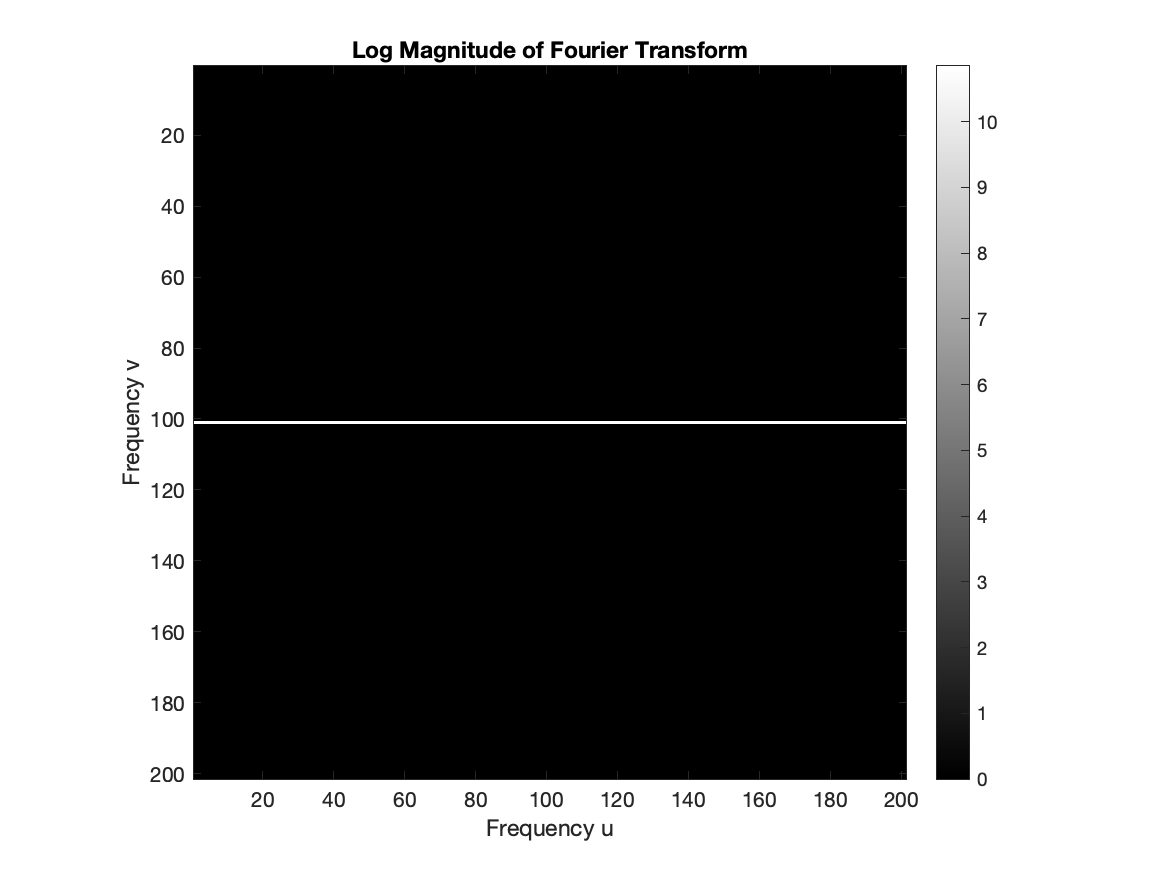
\includegraphics[width=0.8\textwidth]{../images/fourier_log_magnitude_image.png}
    \caption{Log Magnitude of Fourier Transform}
    \label{fig:fft}
\end{figure}



\end{document}